\documentclass{beamer}
%[aspectratio=169]   \usepackage[czech]{babel}
\usepackage{apo-lecture-cz}
\usepackage{pdfpages}
\usepackage{pdfcomment}
\usepackage{listings}
\usepackage{array,multirow}

\subtitle{Lekce 10. Překlad jazyka C}
\author{Pavel Píša \phantom{xxxxxxxxx} Petr Štěpán \\ \small\texttt{pisa@fel.cvut.cz}\phantom{xxxx}\small\texttt{stepan@fel.cvut.cz}}
\begin{document}

\maketitle

\section{Překlad jazyka C}

\begin{frame}
\frametitle{Cíl dnešní přednášky}

\begin{itemize}
 \item Zjistit, jak se program v jazyce C přeloží na strojové instrukce například procesoru RISC-V
 \item Zaměříme se jak se překládá volání funkce
 \item Podíváme se kam se ukládají lokální a globální proměnné
 \item Ukážeme si, jak se liší volání funkcí operačního systému od volání funkcí
\end{itemize}
\end{frame}


\begin{frame}
\frametitle{Jak se překládá program v C}

Jednoduchý příklad -- překlad přiřazení \texttt{a = b + c;}
\begin{enumerate}
 \item Přiřadit proměnným registry, např. b - t0, c - t1, a - t0
 \item Nahrát do registrů hodnoty proměnných: 
 
 \texttt{lw t0, \&b(gp)}; 
 
 \texttt{lw t1, \&c(gp)}
 \item Provést výpočet: 
 
 \texttt{add t0, t0, t1}
 \item Uložit hodnotu do proměnné \texttt{a}: 
 
 \texttt{sw t0, \&a(gp)} 
\end{enumerate}

\bigskip

\begin{itemize}
 \item Obecné výrazy se analyzují pomocí bezkontextových gramatik - definuje všechny výrazy možné v jazyce C.
 \item Výše uvedený překlad je bez optimalizace, uloží hodnotu do proměnné a, v dalším kroku ji může opět nahrávat z paměti třeba i do stejného registru. 
 \item Pokud by adresy proměnných nebyly dosažitelné registrem \texttt{gp}, je nutné před instrukcí \texttt{lw} nahrát adresu proměnné.
\end{itemize}

\end{frame}


\begin{frame}[fragile]
\frametitle{Překlad konstrukce while}

Složitější příklad -- překlad konstrukce \texttt{while (cond) body;}
\begin{columns}
\begin{column}{0.7\textwidth}
\small
\begin{itemize}
 \item analýza bezkontextové gramatiky jazyka detekuje while konstrukci
 \item rekurzivně se zajistí překlad podmínky \texttt{cond} na množinu instrukcí \texttt{COND} a překlad těla cyklu \texttt{body} na množinu instrukcí \texttt{BODY}.
 \item vygeneruje se instrukce \texttt{j cond\_1}, skok na návěstí cond\_1
 \item vloží se návěstí \texttt{body\_1}
 \item vloží se všechny instrukce těla cyklu \texttt{BODY}
 \item vloží se návěstí \texttt{cond\_1}
 \item vloží se instrukce pro generování podmínky \texttt{COND}, výsledek bude např. v registru t0
 \item vygeneruje se instrukce \texttt{bne t0, zero, body\_1}
\end{itemize}
\end{column}
\begin{column}{0.3\textwidth}  
\begin{minted}[fontsize=\footnotesize]{gas}
  j  cond_1
    
body_1:

  BODY

cond_1:

  COND
    
  bne t0, zero, body_1
\end{minted}
\end{column}
\end{columns}

\end{frame}


\begin{frame}
\frametitle{Proč se zabývat překladem?}

\begin{itemize}
 \item Buď používáte interpretované jazyky, které jsou ze své podstaty pomalejší 
 \begin{itemize}
 \item rychlejší jsou pouze, pokud využívají knihovny přeložené do strojových instrukcí a většinou velmi optimalizované např. OpenCV, NumPy, TensorFlow,  PyTorch apod.
 \end{itemize}
 \item nebo používáte překládané jazyky, jako je C/C++, Rust, Fortran, Pascal a pak neběží program v C, ale program přeložený do strojových instrukcí. 
 \item Pokud nevíte, jak se program přeloží:
\begin{itemize}
 \item plně spoléháte na překladač a jeho optimalizace
 \item nadefinujete si ve funkci pole o velikostech 100MiB
 \item bude používat rekurzi, i když neznáte hloubku této rekurze
\end{itemize}
\item V domácím úkolu 4 si procvičíte analýzu strojového kódu a zkusíte si napsat C program, který se bude chovat obdobně (ideálním cílem by bylo, že se přeloží do zadaného kódu strojových instrukcí). 
\end{itemize}
\end{frame}


\begin{frame}
\frametitle{Jak se přeloží funkce?}

Pro překlad funkce např. \texttt{int secti(int a, int b);} je nutné vymyslet:
\begin{itemize}
 \item Jak předat parametry a,b?
 \item Jak předat výsledek secti?
 \item Jakou instrukci dát na konec funkce, kam skočit?
\end{itemize}

Volající (caller) a volaný (callee) se musí dohodnout na těchto otázkách, aby si rozuměli.
\begin{itemize}
 \item Překlad volaného může být na jiném počítači, jiným překladačem (typicky knihovny) než překlad volajícího - Vaším překladačem na Vašem počítači.
 \item Je nutné definovat konvenci, typ konvence volání funkce musí být v hlavičce objektových souborů (a tím i knihoven) aby zajistila správnost předání dat a získání návratové hodnoty funkce.
\end{itemize}
\end{frame}

\section{Konvence volání funkce pro RISC-V}

\begin{frame}[fragile]
\frametitle{Konvence volání funkce pro RISC-V}

\begin{itemize}
 \item Parametry funkce uloží volající do registrů \texttt{a0}, ... , \texttt{a7}
\begin{itemize}
 \item Co když bude parametrů více? Probereme v této přednášce později.
\end{itemize}
 \item Výsledek funkce bude v registrech \texttt{a0} a \texttt{a1}.
\begin{itemize}
 \item Co když se výsledek nevejde do těchto dvou registrů?
 \item Volající musí připravit místo, kam se výsledek uloží.
 \item Ukazatel na adresu výsledku předá jako skrytý parametr do funkce.
 \item Volaný uloží výsledek funkce rovnou na připravenou adresu.
\end{itemize}
\end{itemize}

\begin{columns}
\begin{column}{0.45\textwidth}  
\begin{minted}[fontsize=\footnotesize]{c}
struct a {
  int a, b, c, d;
};

struct a permut(int x, int y);

struct a t;

t = permut(2, 3);
\end{minted}
\end{column}
\begin{column}{0.55\textwidth}  
\begin{minted}[fontsize=\footnotesize]{c}
struct a {
  int a, b, c, d;
};

void permut(struct a *r, int x, int y);

struct a t;

permut(&t, 2, 3);
\end{minted}
\end{column}
\end{columns}
\end{frame}


\begin{frame}[fragile]
\frametitle{Jak přeložit návrat z funkce?}

\begin{columns}
\begin{column}{0.3\textwidth}  
\begin{minted}[fontsize=\footnotesize]{gas}
[0x100]  j  soucet
         
         ...
         
[0x254]  j  soucet
    

soucet:

    ...
    
    j ? 
0x104 nebo 0x258?
nebo jinam
\end{minted}
\end{column}
\begin{column}{0.7\textwidth}
\begin{itemize}
 \item funkce soucet může být volána z mnoha různých míst programu
 \item nelze vygenerovat adresu skoku návrat z funkce v době překladu
 \item návratová adresa musí být nastavena volajícím
 \item konvence volání funkce -- návratová adresa je uložena v registru \texttt{ra} (return address) -- registr \texttt{x1}
 \item potřebujeme instrukci, která skočí na adresu uloženou v registru
 \item hodila by se i instrukce, která uloží do registru ra adresu následující instrukce
\end{itemize}
\end{column}
\end{columns}
\end{frame}



\begin{frame}
\frametitle{Instrukce jal, jalr (ret, jr)}

Instrukce \texttt{jal \textit{[rd,]} address}
\begin{itemize}
 \item skoč na adresu \texttt{address} a do registru \texttt{rd} ulož hodnotu \texttt{PC}+4
 \item pokud neuvedete registr \textit{rd}, tak se standardně doplní \texttt{x1}
 \item pokud chceme jen skok (instrukce \texttt{j}), tak se \texttt{PC}+4 uloží do registru \texttt{x0}
 \item cíl je kódovaný relativně, 21 bitů znaménkově rozšířený posun se přičte k \texttt{PC}/adrese instrukce \texttt{jal}, nejnižší bit fixně 0, maximální vzdálenost $\pm$1\,MB
\end{itemize}

Instrukce \texttt{jalr \textit{rd}, \textit{rs1}, imm12}
\begin{itemize}
 \item skoč na adresu \textit{rs1} + imm12 a do registru rd ulož hodnotu \texttt{PC}+4
 \item pokud neuvedete registr \textit{rd}, tak se standardně doplní \texttt{x1}
 \item pokud chceme jen návrat z funkce, lze použít pro rd registr \texttt{x0}
\end{itemize}
\end{frame}


\begin{frame}
\frametitle{Implemetace jal a jalr}

\begin{center}

\includegraphics[width=0.9\textwidth]{Qtrvsim-jalr.pdf}
\end{center}

Kvíz: Kolik různých čar byste uměli vysvětlit

\phantom{Kvíz: }A -- žádnou B -- asi třetinu  C -- asi polovinu D -- téměř všechny.
\end{frame}


\begin{frame}
\frametitle{Simulace Jalr}

\begin{center}

\includegraphics[width=0.9\textwidth]{Jalr-exec.pdf}
\end{center}

\end{frame}



\begin{frame}
\frametitle{Řídicí hazard při Implemetaci jalr}

\begin{center}

\includegraphics[width=0.9\textwidth]{Jalr-mem.pdf}
\end{center}

\end{frame}



\begin{frame}
\frametitle{Co když funkce ve svém těle volá jinou funkci?}

Volající připraví argumenty do registrů \texttt{a0} až \texttt{a7} a do registru ra návratovou adresu.

\bigskip

Jak ale vyřešit, když funkce ve svém těle volá jinou funkci?

\bigskip

Je nutné někam uložit registr \texttt{ra}, registry \texttt{a0}--\texttt{a7}, ale kam?


\begin{itemize}
 \item Pro uložení dočasných proměnných slouží: Activation record nebo také activation frame. 
 \item Tento záznam, nebo rámec se uloží na zásobník (anglicky call stack nebo stack frame).
\end{itemize}
\end{frame}


\begin{frame}
\frametitle{Zásobník}

\begin{columns}
\begin{column}{0.7\textwidth}
Zásobník je datová struktura LIFO (Last In First Out) -- neboli poslední vložená data jdou první ven
\begin{itemize}
 \item push -- vlož data do zásobníku
 \item pop -- vyber data ze zásobníku
\end{itemize}

Implemetace zásobníku registrem \texttt{sp} (\texttt{x2}):
\begin{itemize}
 \item push 
 
\texttt{addi sp, sp, -4 \phantom{xx}}  -- alokace místa

\texttt{sw \phantom{xx}x10, 0(sp) \phantom{xx}}  -- uložení hodnoty
 
 \item pop

\texttt{lw \phantom{xx}x10, 0(sp) \phantom{xx}}  -- načtení hodnoty

\texttt{addi sp, sp, 4 \phantom{xxx}}  -- dealokace místa

\end{itemize}

\end{column}
\hfill
\begin{column}{0.3\textwidth}  
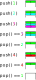
\includegraphics[width=0.9\textwidth]{stack-push-pop.pdf}
\end{column}
\end{columns}

\end{frame}

\begin{frame}
\frametitle{Co se ukládá na zásobník?}

Activation frame obsahuje:
\begin{itemize}
 \item Parametry funkce a návratová adresa, pokud se v těle funkce volá jiná funkce.
 \item Lokální proměnné funkce, které existují jen v průběhu vykonávání funkce.
 \item Podle konvence překladu funkce se nesmí po návratu z funkce změnit hodnota registrů \texttt{s0}--\texttt{s11}
\begin{itemize}
 \item Registr \texttt{s0} se někdy používá jako ukazatel na Activation frame a nazývá se \texttt{fp} -- frame pointer
 \item Registr \texttt{fp} se využívá jako pevný ukazatel na předem dané místo rámce a tím ho lze použít k odkazu na lokální proměnné funkce a parametry funkcí.
\end{itemize}
\end{itemize}
\end{frame}


\begin{frame}
\frametitle{Konvence volání funkce}

Tabulka popisuje jak registry nastavuje volající (caller), volaný (callee)
a pro které je zaručené, že zůstanou pro volajícího nezměněné.

\begin{tabular}{|c|c|p{4cm}|c|c|}\hline
Symbol. & Registr & Popis & Ukládá & Zacho- \\
   jméno   &         &       &        & vaný \\ \hline
zero & x0 & fixní nula/ignorovaný &  -- -- & --\\\hline
a0 - a7 & x10 - x17 & vstupní parametry funkce / dočasné & volající & ne\\\hline
a0, a1 & x10, x11 & výstupní hodnota funkce & volaný & ne\\\hline
ra & x1 & návratová adresa & volající & ano\\\hline
t0 - t6 & x5-7, x28-x31 & dočasné registry & volající & ne\\\hline
s0 - s11 & x8-9, x18-x27 & ukládané registry & volaný & ano\\\hline
sp & x2 & ukazatel zásobníku & volaný & ano\\\hline
gp & x3 & globální ukazatel & -- -- & ano\\\hline
tp & x4 & ukazatel na vlákno (thread) & -- -- & ano\\\hline
\end{tabular}
\end{frame}


\begin{frame}
\frametitle{Konvence volání funkce na 32 bitovém RISC-V systému}

\begin{itemize}
 \item Standard: 32-bit RISC-V Calling Convention
 \item char, short, int, long, float, pointer -- každý parametr jeden registr
 \item long long int, double -- každý parametr dva registry (první registr má sudé číslo)
 \item struct předávaná hodnotou se kopíruje do tolika registrů, kolik je potřeba
 \item pokud je překládáno pro RISC-V s rozšířením pro práci s reálnými čísly, pak se pro předávání float, double i struktur využijí registry \texttt{f10}--\texttt{f17} označovaných také \texttt{fa0}--\texttt{fa7}
 \item pokud se parametry nevejdou do registrů \texttt{a0}--\texttt{a7}, tak se přebývající parametry umístí na zásobník do rámce nově volané funkce
  \item zásobník musí v době, kdy je funkce volaná (instrukce \texttt{jal}/\texttt{jalr} vykonaná), být zarovnaný na násobek 16 bytů 
\end{itemize}
\end{frame}


\begin{frame}
\frametitle{Kvíz}

Kdy se parametry funkce, nebo registry s0-s11 uloží na zásobník?
\begin{itemize}
 \item[A] nikdy.
 \item[B] když se v těle funkce uloží do parametru jiná hodnota.
 \item[C] když bude v těle funkce volání jiné funkce se stejným počtem parametrů.
 \item[D] když bude v těle funkce použit vstupní parametr po volání funkce.
\end{itemize}
\end{frame}


\begin{frame}
\frametitle{Kvíz}

Kdy se lokální proměnné, nebo registry s0-s11 uloží na zásobník?
\begin{itemize}
 \item[A] nikdy.
 \item[B] když se v těle funkce bude využívat tolik lokálních proměnných, že se jejich hodnoty nevejdou do registrů.
 \item[C] když bude v těle funkce volání jiné funkce.
 \item[D] pouze když bude v těle funkce rekurzivní volání té samé funkce.
\end{itemize}
\end{frame}


\begin{frame}[fragile]
\frametitle{Volání funkce}

\begin{columns}
\begin{column}{0.5\textwidth}
Volání funkce s maximálně 8 parametry:

\begin{minted}[fontsize=\footnotesize]{c}
t = secti(1, 2, 3, 4);
\end{minted}

Překlad do RISC-V
\begin{minted}[fontsize=\footnotesize]{gas}
li  a3,4
li  a2,3
li  a1,2
li  a0,1
jal ra,10054 <secti>
\end{minted}

\end{column}
\begin{column}{0.5\textwidth}  
Volání funkce s 10 parametry:

\begin{minted}[fontsize=\footnotesize]{c}
t = secti(1, 2, 3, 4, 5, 
          6, 7, 8, 9, 10);
\end{minted}

Překlad do RISC-V
\begin{minted}[fontsize=\footnotesize]{gas}
li  a5,10
sw  a5,4(sp)
li  a5,9
sw  a5,0(sp)
li  a7,8
li  a6,7
li  a5,6
li  a4,5
li  a3,4
li  a2,3
li  a1,2
li  a0,1
jal ra,10054 <secti>
\end{minted}
\end{column}
\end{columns}
\end{frame}




\begin{frame}
\frametitle{Překlad funkce - jednoduchá funkce}

Příklad s málo parametry bez vnitřního volání funkce se čtyřmi lokálními proměnnými.
\begin{columns}
\begin{column}{0.65\textwidth}
\begin{itemize}
 \item Alokace místa pro lokální proměnné 
 
 \texttt{addi  sp,sp,-16}
 \item Lokální proměnné na adresách: 
 
 0(sp), 4(sp), 8(sp), 12(sp)
\begin{itemize}
 \item Pokud to lze, jsou proměnné umístěny v registrech a stack by se vůbec nepoužil
\end{itemize}
\end{itemize}

Ukončení funkce:
\begin{itemize}
 \item Dealokace místa pro lokální proměnné 
 
 \texttt{addi  sp,sp,16}
 \item Návrat z funkce 
 
 \texttt{jalr 0(x1)} -- \texttt{ret} 
\end{itemize}
\end{column}
\begin{column}{0.35\textwidth}  
\includegraphics[width=0.9\textwidth]{simple_fnc-cz.pdf}
\end{column}
\end{columns}

\end{frame}


\begin{frame}[fragile,shrink=5]
\frametitle{Překlad funkce}

Příklad s 10 parametry, volání funkce uvnitř funkce, se dvěma lokálními proměnnými.

\begin{columns}
\begin{column}{0.35\textwidth}
Začátek funkce (prolog):

\begin{minted}[fontsize=\footnotesize]{gas}
addi  sp,sp,-48
sw  ra,44(sp)
sw  s0,40(sp)
sw  s1,36(sp)
sw  s2,32(sp)
sw  s3,28(sp)
sw  s4,24(sp)
\end{minted}

Lokální proměnné:
\begin{minted}[fontsize=\footnotesize]{gas}
lw  t0,8(sp)
lbu t1,15(sp)
\end{minted}

\texttt{int i;} na adrese 8(\texttt{sp})

\texttt{char c;} na adrese 15(\texttt{sp})

0(\texttt{sp}) -- 7(\texttt{sp}) nevyužito nebo rezervované pro volání uvnitř funkce


\end{column}
\begin{column}{0.29\textwidth}
Ukončení funkce (epilog):

\begin{minted}[fontsize=\footnotesize]{gas}
lw   ra,44(sp)
lw   s0,40(sp)
lw   s1,36(sp)
lw   s2,32(sp)
lw   s3,28(sp)
lw   s4,24(sp)
addi sp,sp,48
ret
\end{minted}
Poznámka: alokace zásobníku je zarovnaná na 16 bytů.

\end{column}
\begin{column}{0.35\textwidth}  
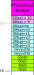
\includegraphics[width=0.7\textwidth]{complex_fnc-cz.pdf}
\end{column}
\end{columns}
\end{frame}


\begin{frame}[shrink=5]
\frametitle{Ukazatel na rámec funkce}

\begin{itemize}
 \item Ukazatel na rámec funkce obsahuje v RISC-V hodnotu sp při vstupu do funkce
 \item Pro \texttt{fp} (frame pointer) je využit registr \texttt{s0}, je to tedy registr, který musí volaný uložit a při návratu z funkce obnovit
 \item Výhody použití \texttt{fp}
\begin{itemize}
 \item Pevně nastavené ukazatele na argumenty a lokální proměnné funkce, pokud se sp v těle mění (např. argumenty pro volné funkce), pak se mění i posunutí vzhledem k sp pro přístup k argumentům a lokálním funkcím.
 \item Přehlednější zásobník pro debugery a při tzv. odvinutí zásobníku.
\begin{itemize}
 \item Odvinutí zásobníku se provádí v C++ při výskytu výjimky ve funkci, kdy je ale výjimka zpracována až ve funkci nadřazené, která tuto funkci volala.
 \item Pro zpracování výjimky je nutné nastavit zásobník do stavu, ve které nadřazená funkce volala funkci, ve které výjimka nastala.
\end{itemize}
\end{itemize}
 \item Nevýhody použití \texttt{fp}:
\begin{itemize}
 \item Zpomaluje program, jedná se sice jen o několik instrukcí při vstupu a ukončení funkce, ale pokud se funkce volá často a její tělo je krátké, může to být i značné zpomalení.
 \item Fp obsadí registr s0, který by se dal využít pro uchování hodnoty. Pokud by došly volné registry, pak se hodnota musí uložit na zásobník do paměti RAM (přes cache), což je pomalejší než využití registru.
\end{itemize}
\end{itemize}
\end{frame}


\begin{frame}[fragile,shrink=5]
\frametitle{Překlad funkce s ukazatelem na rámec funkce}

Pro překlad s vynuceným používáním \texttt{fp} pro RISC-V je nutné využít GCC přepínač \texttt{-fno-omit-frame-pointer}
\begin{columns}
\begin{column}{0.25\textwidth}
Začátek funkce v~případě RISC-V:

\begin{minted}[fontsize=\footnotesize]{gas}
addi sp,sp,-48
sw   ra,44(sp)
sw   s0,40(sp)
sw   s1,36(sp)
sw   s2,32(sp)
sw   s3,28(sp)
sw   s4,24(sp)
sw   s5,20(sp)
addi s0,sp,48
\end{minted}
\end{column}   
\begin{column}{0.4\textwidth}
Odkaz na lokální proměnnou:

\begin{minted}[fontsize=\footnotesize]{gas}
sw a0,-36(s0)
\end{minted}
dříve:
\begin{minted}[fontsize=\footnotesize]{gas}
sw a0, 12(sp)
\end{minted}



Ukončení funkce:

\begin{minted}[fontsize=\footnotesize]{gas}
lw   ra,44(sp)
lw   s0,40(sp)
lw   s1,36(sp)
lw   s2,32(sp)
lw   s3,28(sp)
lw   s4,24(sp)
lw   s5,20(sp)
addi sp,sp,48
ret
\end{minted}
\end{column}
\begin{column}{0.35\textwidth}  
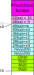
\includegraphics[width=0.7\textwidth]{complex_fnc_fp-cz.pdf}
\end{column}
\end{columns}
\end{frame}


\begin{frame}[fragile,shrink=5]
\frametitle{Řešení domácího úkolu 4}

Analyzovat funkci \texttt{subroutine\_fnc}:
\begin{itemize}
\item zjistit, jaké registry \texttt{a0} -- \texttt{a7} se ve funkci používají a jaké se před volání funkce naplní
 \begin{itemize}
 \item POZOR překladač využívá registry \texttt{a\textit{X}} také pro pomocné výpočty stejně jako registry \texttt{t0} -- \texttt{t6}, protože jejich hodnoty může měnit
 \end{itemize}
\item zjistit, co je v registru \texttt{a0} před zavoláním instrukce \texttt{ret} (\texttt{jalr 0(x1)})
\item prozkoumat začátek funkce:
 \begin{itemize}
 \item pokud funkce začíná sekvencí instrukcí podobné:
\begin{minted}[fontsize=\footnotesize]{gas}
addi  sp,sp,-48
sw  ra,44(sp)
sw  s0,40(sp)
sw  s1,36(sp)
sw  s2,32(sp)
sw  s3,28(sp)
sw  s4,24(sp)
\end{minted}
\begin{itemize}
 \item pak funkce využívá zásobník pro uložení návratové adresy a lokálních dat
 \item adresy od 0(\texttt{sp}) do 23(\texttt{sp}) jsou využity pro lokální proměnné funkce
 \item registry \texttt{s0} -- \texttt{s4} (v tomto případě) jsou využity pro uchování dočasných hodnot, pravděpodobně argumentů funkce
 \end{itemize}
 \item pokud funkce neobsahuje instrukci \texttt{addi sp,sp,-X} pak se jedná o "jednoduchou" funkci, která nepoužívá zásobník
\begin{itemize}
 \item všechny lokální proměnné a mezivýpočty jsou uloženy v nepoužitých registrech \texttt{a0} -- \texttt{a7} a registrech \texttt{t0} -- \texttt{t6}
 \end{itemize}
 \end{itemize}
 \end{itemize}
\end{frame}


\begin{frame}
\frametitle{Rozložení běžícího programu v paměti}

\begin{columns}
\begin{column}{0.75\textwidth}
Každý proces má pro sebe 4GiB virtuálního prostoru:
\small
\begin{itemize}
\item Nejvyšší 1GiB má pro sebe operační systém
\item Následuje zásobník (pokud má proces více vláken, pak jsou zásobníky dalších vláken většinou alokované z~haldy)
\item Níže jsou dynamické knihovny
\item Od globálních dat (\texttt{.data}+\texttt{.bss}) roste dynamicky alokovaná paměť -- heap (malloc,new/free,delete)
\item Globální data (inicializovaná \texttt{.data} i neinicializovaná \texttt{.bss})
\item Program (\texttt{.text})
\item Adresy od 0 se nechávají neobsazené kvůli odchytávání chyby dereference NULL ukazatele.
\end{itemize}
\end{column}   
\begin{column}{0.25\textwidth}  
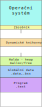
\includegraphics[width=0.8\textwidth]{proc_addr_space-cz.pdf}
\end{column}
\end{columns}
\end{frame}

\begin{frame}[fragile,shrink=5]
\frametitle{Řešení domácího úkolu 4}

Využití globálních proměnných:
\begin{itemize}
\item globální proměnná je proměnná definovaná mimo funkci, nebo uvnitř funkce s použitím klíčového slova \texttt{static}
\item globální inicializované proměnné jsou umístěné v sekci .data, neinicializované proměnné v sekci .bss
\item Jak zjistit, zda v mém programu jsou globální proměnné?
 \begin{itemize}
 \item podívejte se na konec výpisu riscv assembleru a najděte sekci \texttt{my\_data}.
 
 Tato sekce může vypadat takto:
\begin{minted}[fontsize=\footnotesize]{gas}
Contents of section my_data:
    11008 00000000                ....
\end{minted}
\begin{itemize}
 \item 11008 je adresa dat ve virtuálním prostoru procesu
 \item 00000000 je hexadecimální výpis uložených dat
 \item .... je textový (ASCII) výpis uložených dat, pokud znak nelze zobrazit je místo něj použita tečka
 \item využití dat v programu vypadá takto:
\begin{minted}[fontsize=\footnotesize]{gas}
lui  a5, 0x11
addi a5, a5, 8 # 11008
lw   a4, 0(a5)
\end{minted}
 \end{itemize}
 \end{itemize}
 \end{itemize}
\end{frame}


\begin{frame}[fragile]
\frametitle{Kvíz}

Uvažujte tuto funkci
\begin{minted}[fontsize=\footnotesize]{c}
int fce (int a) {
  int i;
  
  // telo funkce
  
  return i+a;
}
\end{minted}
Kde budou umístěny proměnné \texttt{a} a \texttt{i}:
\begin{itemize}
 \item[A] obě na zásobníku nebo v registrech
 \item[B] obě v datové sekci
 \item[C] \texttt{a} na zásobníku nebo v registru, \texttt{i} v datové sekci
 \item[D] \texttt{a} v datové sekci, \texttt{i} na zásobníku nebo v registru
\end{itemize}
\end{frame}


\begin{frame}[fragile,shrink=5]
\frametitle{Útok na program přes zásobník}

\begin{columns}
\begin{column}{0.42\textwidth}
Uvažujme tento program:

\begin{minted}[fontsize=\footnotesize]{c}
int virus() {
  // skodi
  return 0;
}

int secti(int a, int b, int c, 
  int d, int e, int f, int g, 
  int h, int i, int j) {
  
  volatile int ii,jj=i+j;
  volatile int pole[2];
  
  // neco pocita a
  // vola nejakou funkci
  
  pole[11] = (int)&virus;
  
  return pole[0]+pole[1];
}
\end{minted}
\end{column}   
\begin{column}{0.25\textwidth}
Úvod funkce:

\begin{minted}[fontsize=\footnotesize]{gas}
addi sp,sp,-48
sw   ra,44(sp)
sw   s0,40(sp)
sw   s1,36(sp)
sw   s2,32(sp)
sw   s3,28(sp)
\end{minted}


\begin{minted}[fontsize=\footnotesize]{gas}
# pole[11]=(int)&virus;
lui  a5,0x10
addi a5,a5,84 # <virus>
sw   a5,44(sp)
\end{minted}

Ukončení funkce:

\begin{minted}[fontsize=\footnotesize]{gas}
lw   ra,44(sp)
lw   s0,40(sp)
lw   s1,36(sp)
lw   s2,32(sp)
lw   s3,28(sp)
addi sp,sp,48
ret
\end{minted}
\end{column}
\begin{column}{0.33\textwidth}  
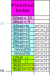
\includegraphics[width=\textwidth]{overflow_fnc-cz.pdf}
\end{column}
\end{columns}
\end{frame}



\begin{frame}[fragile]
\frametitle{Proměnný počet parametrů va\_list}

Definice funkce s proměnným počtem parametrů (variadic function):

\begin{columns}
\begin{column}{0.4\textwidth}
\begin{minted}[fontsize=\footnotesize]{c}
#include <stdarg.h>

int secti(int n, ...) {
  int souc = 0;
  int i;
  va_list ap;
  
  va_start(ap, n);
  for (i=0; i<n; i++) {
    souc+=va_arg(ap,int);
  }
  va_end(ap);
  return souc;
}
\end{minted}
\end{column}   
\begin{column}{0.6\textwidth}
Volání funkce:

\begin{minted}[fontsize=\footnotesize]{c}
int  main() {
  printf("Soucet %d\n", secti(10, 1,2,3,
                         4,5,6,7,8,9,10);
  printf("Soucet %d\n", secti(2, 1,2);
  printf("Soucet %d\n", secti(8, 1,2,3,
                              4,5,6,7,8);
}
\end{minted}
\end{column}
\end{columns}

\end{frame}

\begin{frame}[fragile,shrink=5]
\frametitle{Překlad funkce secti s proměnným počtem parametrů}

Makro \texttt{va\_start} a \texttt{va\_arg} potřebuje mít uloženy všechny parametry v paměti:

\begin{columns}
\begin{column}{0.25\textwidth}
Začátek funkce:

\begin{minted}[fontsize=\footnotesize]{gas}
addi sp,sp,-64
sw   ra,28(sp)
sw   s0,24(sp)
sw   s1,20(sp)
sw   a1,36(sp)
sw   a2,40(sp)
sw   a3,44(sp)
sw   a4,48(sp)
sw   a5,52(sp)
sw   a6,56(sp)
sw   a7,60(sp)
\end{minted}
\end{column}   
\begin{column}{0.4\textwidth}
\texttt{va\_start(ap, n)}:

\begin{minted}[fontsize=\footnotesize]{gas}
addi a5,sp,36
sw   a5,8(sp)
\end{minted}
\texttt{va\_arg(ap, int)}:
\begin{minted}[fontsize=\footnotesize]{gas}
lw   a4,8(sp)
addi a3,a4,4
sw   a3,8(sp)
lw   s0,0(a4)
\end{minted}

Ukončení funkce:

\begin{minted}[fontsize=\footnotesize]{gas}
lw   ra,28(sp)
lw   s0,24(sp)
lw   s1,20(sp)
addi sp,sp,64
ret
\end{minted}
\end{column}
\begin{column}{0.3\textwidth}  
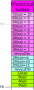
\includegraphics[width=0.7\textwidth]{vaarg_fnc_fp-cz.pdf}
\end{column}
\end{columns}
\end{frame}


\section {Systémová volání}

\begin{frame}
\frametitle{Základy ochrany OS}

\begin{itemize}
\item Uživatelský proces nemůže přímo přistupovat k HW počítače.
\item Uživatelský proces musí požádat OS o zpřístupnění HW, nebo vyřízení požadavku.
\item To co OS umožňuje procesům jsou pouze systémová volání (system calls).
\item Na rozdíl od volání funkce neznáme adresy funkcí v jádře.
\item Systémové volání se vybírá číslem systémového volání.
\item Vlastní zavolání funkce je vyvolání přerušení nebo výjimky specializovanou instrukcí:
\begin{itemize}
\item x86 -- používá přímo int 0x80 -- vyvolej přerušení číslo 0x80.
\item x86 -- nověji specializované instrukce sysenter/syscall -- podobný mechanizmus, ale nevyužívá systémový zásobník, složitý mechanizmus bran a přistupuje k méně paměti $\rightarrow$ je rychlejší.
\item RISC-V -- specializovaná instrukce ecall -- obdobně jako při přerušení.
\end{itemize}
\item Při přerušení/výjimce se volá obslužná rutina v privilegovaném řežimu (typicky systémovém) z adresy, která je nastavená OS (na RISC-V registry \texttt{mtvec}/\texttt{stvec}), uživatel ji nemůže měnit.

\end{itemize}
\end{frame}

\begin{frame}
\frametitle{Ochrana OS}

Uživatelský program nastaví parametry volání do registrů vyvolá speciální přerušení/výjimku (na RISC-V \texttt{ecall}).

OS podle čísla systémového volání zavolá odpovídající funkci.

\begin{center}
  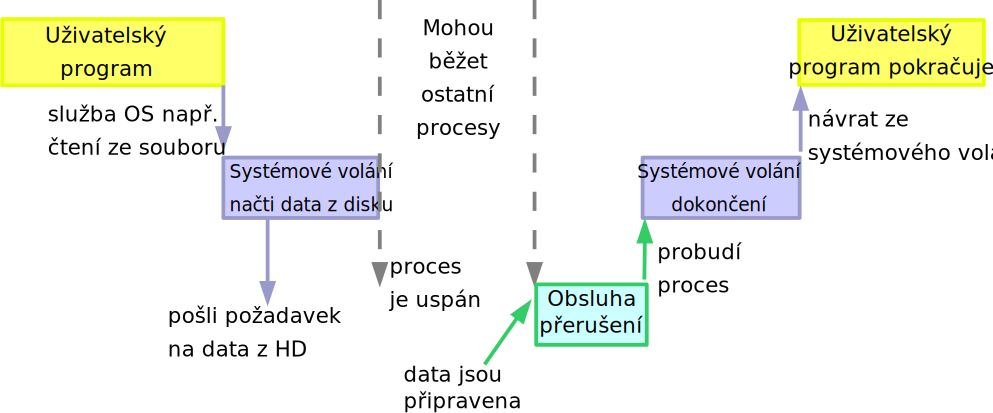
\includegraphics[width=0.95\textwidth]{irq-and-os-cz.pdf}
\end{center}

Návrat ze systémového volání odpovídá návratu z přerušení/výjimky (na RISC-V většinou \texttt{sret}).

\end{frame}

\begin{frame}[shrink=5]
\frametitle{ABI systémového volání}

\begin{itemize}
\item API -- application programming interface -- popis, jaké funkce může Váš program zavolat z knihoven.
\begin{itemize}
\item API je definováno pro jazyk C hlavičkovými soubory.
\item API definuje i co dané funkce dělají, jaké vrací hodnoty, jak se chovají při chybě
\item zkuste např. \texttt{man 2 read}
\end{itemize}
\item ABI -- application binary interface -- popis jaké registry a jaké instrukce použít
\item ABI pro systémová volání na architektuře RISC-V
\begin{itemize}
\item \texttt{a7} -- obsahuje číslo systémového volání (přehled např. \url{https://jborza.com/post/2021-05-11-riscv-linux-syscalls/} nebo \url{https://marcin.juszkiewicz.com.pl/download/tables/syscalls.html})
\item \texttt{a0} až \texttt{a5} -- parametry systémového volání (Linuxové systémové volání má maximálně 6 parametrů)
\item systémové volání se provede instrukcí \texttt{ecall}
\item \texttt{a0} obsahuje návratovou hodnotu systémového volání
\begin{itemize}
\item pokud by mělo vracet více dat (např. čtení ze souboru) musí uživatel zadat ukazetel na buffer a velikost bufferu, kam OS zapíše data.
\end{itemize}
\end{itemize}
\end{itemize}

\end{frame}

\begin{frame}[fragile]
\frametitle{Příklad Hello world!}


\begin{minted}[fontsize=\footnotesize]{gas}
.global _start
.text
_start:
#   write(1, "Hello world!\n", 13);
   addi  a7, zero, 64
   addi  a0, zero, 1
   la    a1, zero, text_1
   addi  a2, zero, 13
   ecall
final:
#   exit(0);
   addi  a7, zero, 93
   addi  a0, zero, 0
   ecall
   ebreak
   j final
.data
# store ASCII text, no termination
text_1: .ascii "Hello world!\n"
\end{minted}
\end{frame}


\begin{frame}[fragile]
\frametitle{Řešení domácího úkolu 4}

Co dělat se systémovým voláním?
\begin{itemize}
\item najděte instrukci \texttt{ecall}.
\item podle hodnotu registru \texttt{a7}, z ní zjistěte o jaké systémové volání se jedná.
\item zjistěte hodnoty registrů \texttt{a0}, \texttt{a1}, \texttt{a2} (případně \texttt{a3} pokud je použit).
\item do C programu zařaďte volání funkce z API, která provede dané systémové volání.
\item Příklad: zjistíte, že registr \texttt{a7} má hodnotu 63 -- \texttt{read}, vygenerujete volání funkce read
\begin{minted}[fontsize=\footnotesize]{c}
read(a0, a1, a2);
\end{minted}
\begin{itemize}
 \item jediný problém je s funkcí \texttt{open}/\texttt{openat}, jejíž parametry mají jiné hodnoty příznaků \texttt{O\_\textit{XXXX}} pro systém x86 a pro riscv
 \item protože programy kontroluje Brute na systému x86, je lepší ověřit hodnoty parametrů ve výpisu program-x86.list
 \end{itemize}
\end{itemize}
\end{frame}

\begin{frame}
\frametitle{Systémové volání x86}

\begin{itemize}
\item systémové volání provádí instrukce \texttt{int 0x80}.
\item číslo systémového volání je v registru eax.
 \begin{itemize}
 \item POZOR čísla systémových volání x86 a riscv se liší.
 \end{itemize}
\item parametry systémového volání jsou uloženy postupně v registrech:
 \begin{itemize}
 \item ebx 
 \item ecx 
 \item edx 
 \item esi 
 \item edi 
 \item ebp 
 \end{itemize}
\item příští přednášku si probereme assembler x86, abyste mohli využít pro řešení domácího úkolu 4 i výpis instrukcí pro procesor x86.
\end{itemize}
\end{frame}


\begin{frame}[fragile]
\frametitle{Kvíz za bonusový bod}

Uvažujte tuto funkci
\begin{minted}[fontsize=\footnotesize]{c}
int fce (int a) {
  static int s;
  int i;
  
  // telo funkce
  
  return i+s;
}
\end{minted}
Kde budou umístěny proměnné \texttt{s} a \texttt{i}:
\begin{itemize}
 \item[A] obě na zásobníku
 \item[B] obě v datové sekci
 \item[C] \texttt{s} na zásobníku, \texttt{i} v datové sekci
 \item[D] \texttt{s} v datové sekci, \texttt{i} na zásobníku
\end{itemize}
\end{frame}


\end{document}

